\chapter{Estado}

O objetivo do diagrama de estado é descrever como um objeto ou entidade passa por
diferentes estados em resposta a eventos em condições específicas.

Este diagrama de estado considera os objetos da classe ``Evento Agendado''
(ScheduleEvent) e foi cuidadosamente elaborado para modelar e visualizar o ciclo
de vida de um evento na agenda de um usuário. Este diagrama inclui quatro estados
principais: ``Agendado'', ``Finalizado'', ``Expirado'' e ``Cancelado'', cada um
representando um estado específico pelo qual um evento no calendário pode passar
ao longo do tempo. Além disso, o diagrama também incorpora quatro eventos
fundamentais que desencadeiam transições entre esses estados: ``Adicionar Evento'',
``Evento Realizado'', ``Fim do Dia'' e ``Remover Evento''.

\begin{figure}[h]
  \centering
  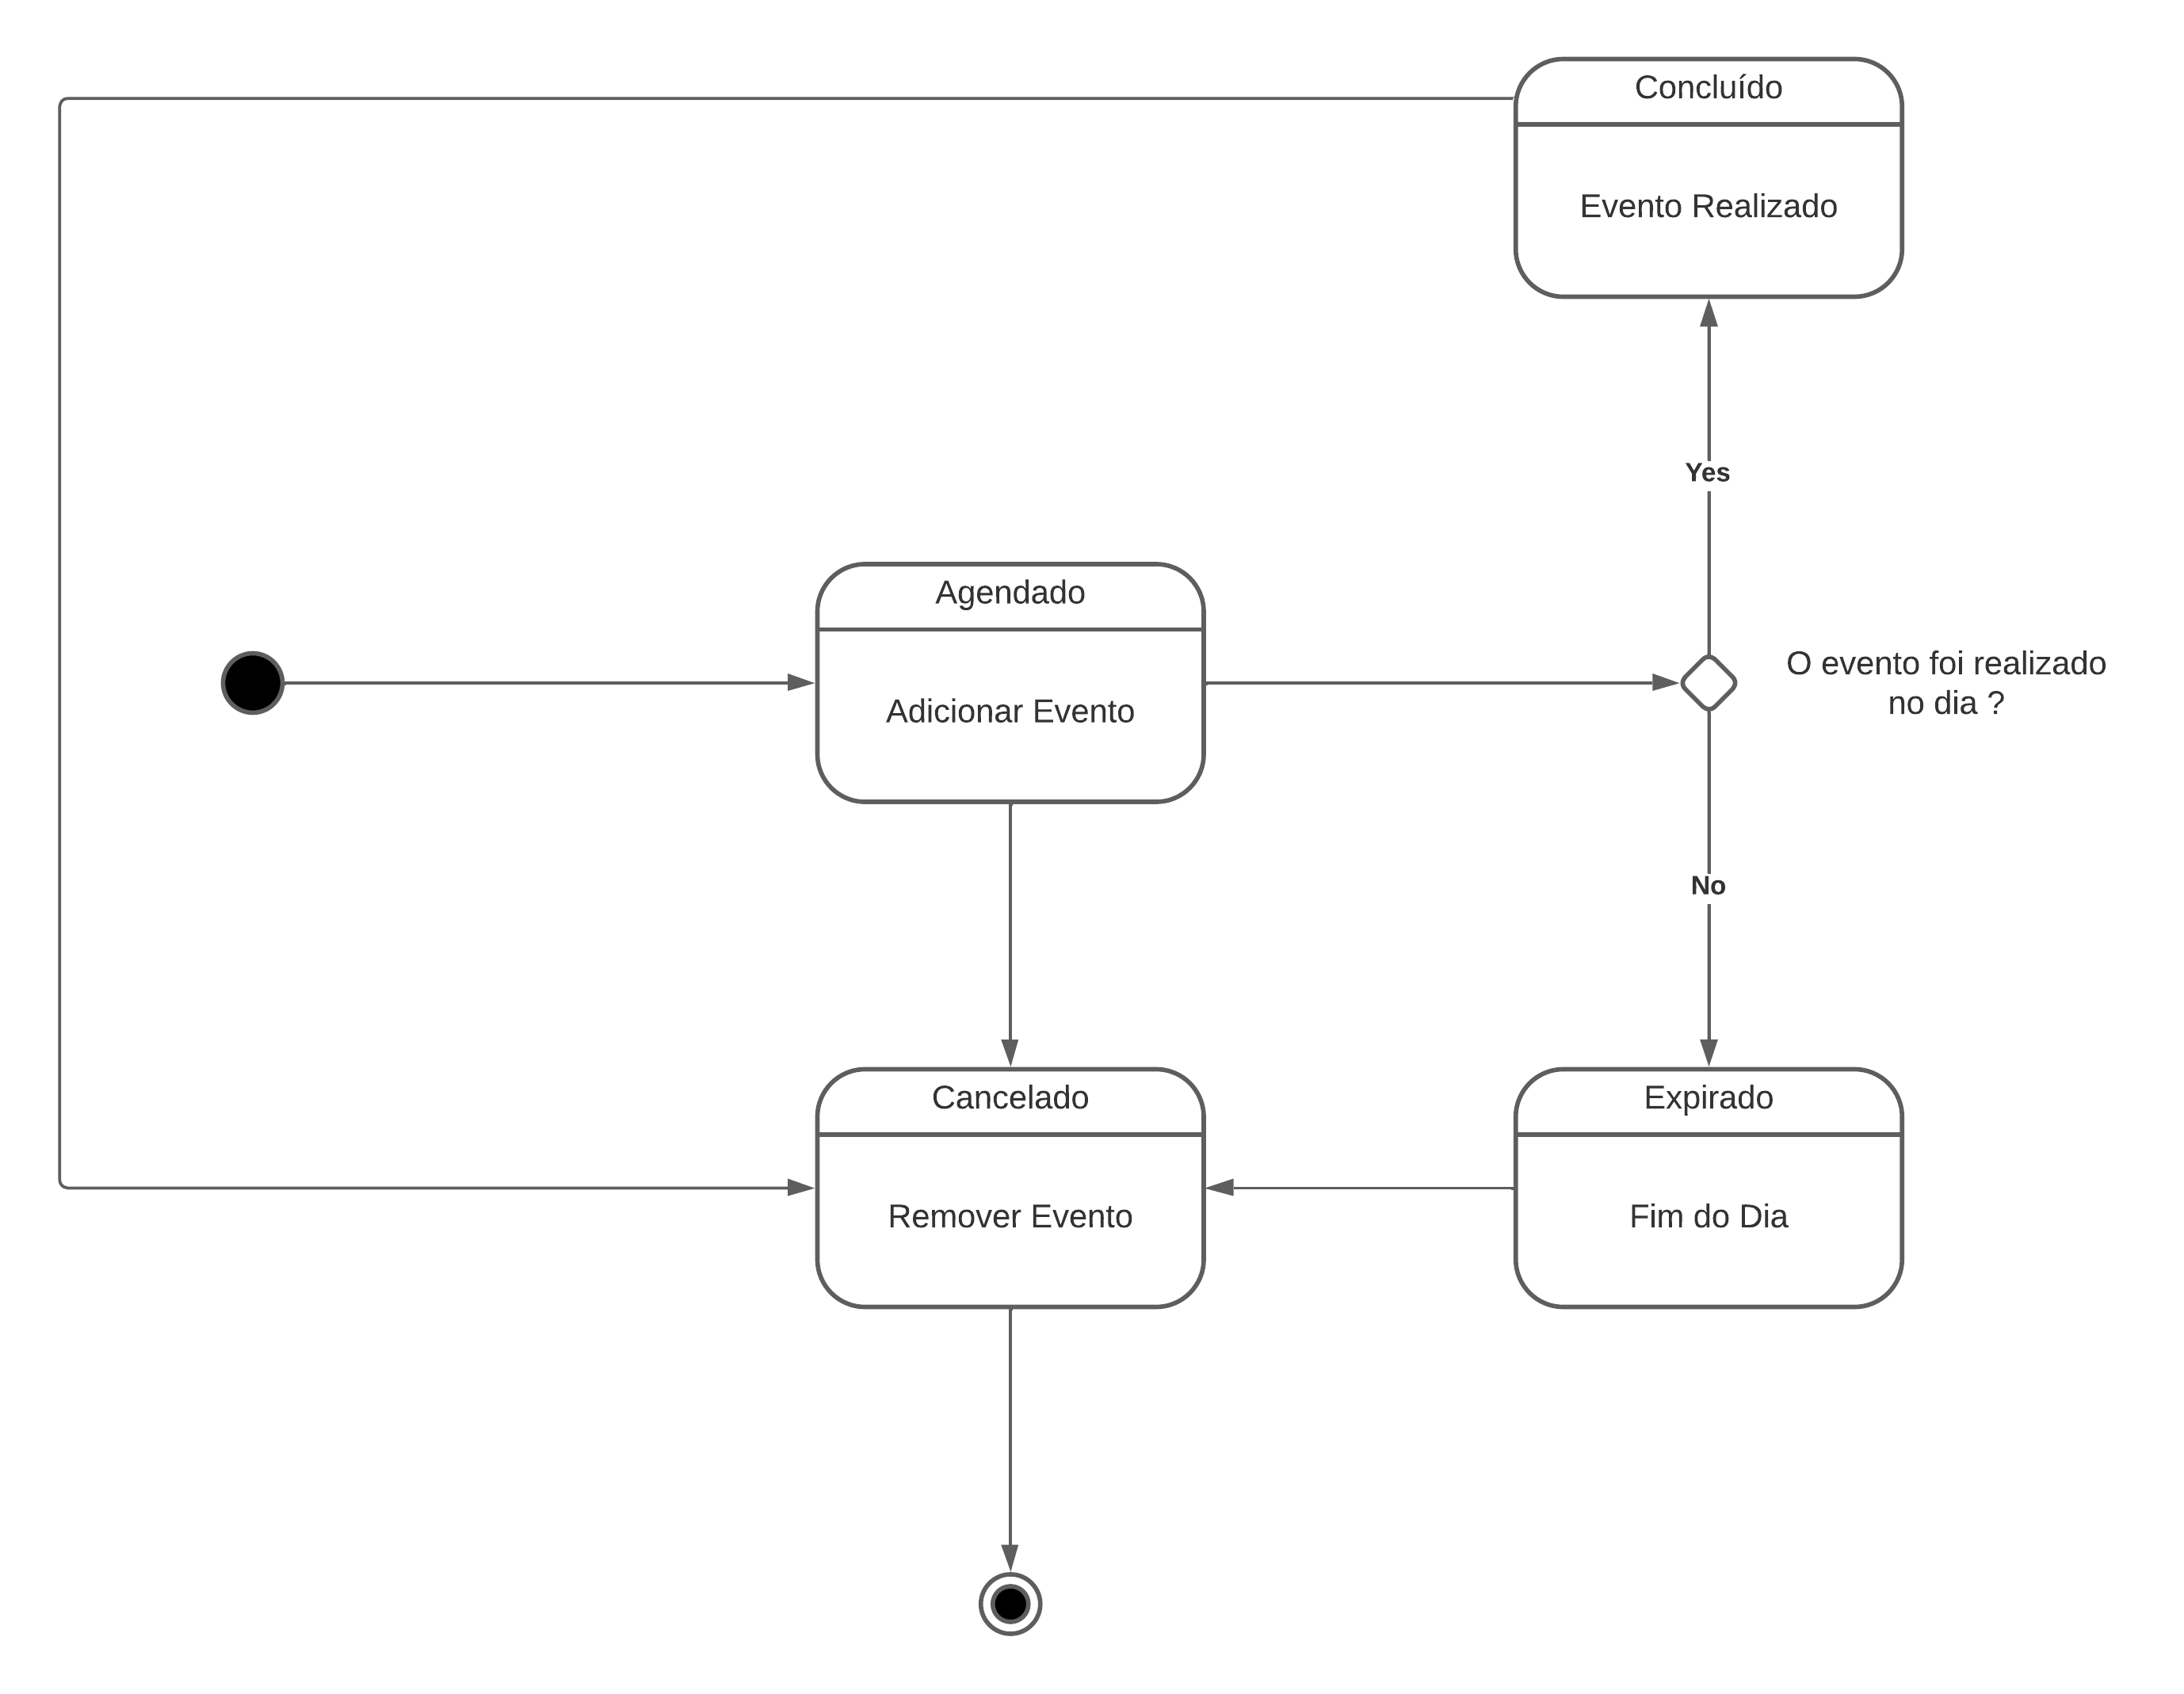
\includegraphics[scale=0.5]{images/diagrams/state.png}
\end{figure}

O estado ``Agendado'' representa o ponto de partida, indicando que um novo evento
foi criado na agenda do usuário. Quando o evento ``Adicionar Evento'' ocorre, o
evento agendado entra no estado de ``Agendado''.

O estado ``Finalizado'' indica que o evento da agenda foi realizado com sucesso e
contabilizado no sistema. O evento ``Evento Realizado'' troca o estado para ``Finalizado''.

O estado ``Expirado'' mostra que o evento da agenda não foi realizado no dia planejado.
O evento ``Fim do Dia'' atualiza o estado para ``Expirado'' caso ainda não esteja
``Finalizado''.

O estado ``Cancelado'' mostra que o evento foi desagendado, ou seja, removido do
agenda. O evento ``Remover Evento'' realiza essa alteração para ``Cancelado''.
